\chapter{Introduction}

The Research Institute \v{R}e\v{z} conducts numerous projects in the nuclear industry. Some of these involve electron microscopy and the analysis of materials subjected to high temperatures and aggressive environments, such as those found in nuclear reactors. A significant portion of these projects requires extensive manual image analysis, making automation a crucial challenge. Currently, image analysis is performed using various processing tools, including Fiji~\cite{Schindelin2012} by ImageJ. This thesis aims to automate one of these manual processes.

The primary focus of this work is the segmentation of coating layers in material samples. These images contain both coating and oxidation layers, with coating layers exhibiting greater uniformity, whereas oxidation layers present irregular structures, as illustrated in Figure~\ref{fig:coating-oxidation}. By initially addressing the segmentation of coating layers, this thesis evaluates the potential of automation in reducing analysis time while maintaining sufficient accuracy. If successful, future work could extend this approach to more complex cases, such as samples without coating layers and those with multiple oxidation types.

Three computer vision algorithms are explored to achieve segmentation, ranging from traditional clustering techniques to advanced deep-learning models. The first method explored is K-means clustering, an unsupervised algorithm that does not require labeled data. While K-means provides a lightweight approach, its effectiveness is hindered by the non-homogeneous nature of coating layers. Due to variations in layers, colors, and structures, different parameter settings must be adjusted for each image, limiting its practical usability. Further details on this method are discussed in Section~\ref{sec:kmeans}.

The second approach involves Convolutional Neural Networks (CNNs), which, unlike K-means, require labeled data and are computationally more demanding. However, CNNs offer good segmentation accuracy once trained. This thesis examines three levels of label precision, balancing annotation effort with segmentation performance. The original labeling come in the form of information about the thinkers of the coating layer at 10 places per picture. From this can be easily reconstructed polygon labels which are not that precise. On the other hand the creation of more precise labels requires extra time of the scientist on top of clacical labeling ith 10 lines. Although the most precise labels yield the best results, less precise labels provide comparable outcomes while significantly reducing annotation time, as discussed in Section~\ref{sec:cnn}.

A major limitation of CNN-based methods is the computational cost of prediction. The available hardware lacks sufficient memory for complex image processing, leading to slow predictions, particularly when relying on CPU computation. Under the current setup, a single prediction requires approximately 14 seconds, compared to around one minute for manual segmentation. Thus, the trade-off between segmentation accuracy and computational efficiency remains a key consideration.

The "Segment Anything" (SAM) model \cite{kirillov2023segany} represents a state-of-the-art approach in image segmentation, leveraging transformers. While SAM holds significant potential to improve segmentation performance, it comes with considerably higher computational demands due to its robustness and the large number of parameters involved. Specifically, the number of parameters in the SAM model and U-Net in this thesis was measured, with the SAM model containing over 21 times more parameters than U-Net. This substantial increase in model complexity leads to a corresponding rise in hardware requirements during predictions. Consequently, the computational demands of the SAM model exceed the capabilities of the available hardware, particularly in the absence of GPU infrastructure. As a result, fine-tuning and evaluating the SAM model was not pursued in this thesis. However, as hardware resources continue to improve, this approach may become a viable option for future research.

In the following chapters, the thesis will focus on the use of K-Means clustering and label creation to develop a cohesive dataset for CNNs with U-Net architecture. It will also address the training and optimization of the model's hyperparameters. Ultimately, the best-performing model will be integrated into the research workflow, and the results obtained by the researcher using this model will be evaluated.



 % the SAM model contains approximately 641 million parameters (measured in jupyter notebook, but on site they say it is 632M for the initial first image encoder https://segment-anything.com/), which is over 21 times more than the 29.9 million parameters in the U-Net model used in this thesis. I tried it with https://stackoverflow.com/questions/49201236/check-the-total-number-of-parameters-in-a-pytorch-model

\begin{figure}[H]
    \centering
    \begin{subfigure}{0.40\textwidth}
        \centering
        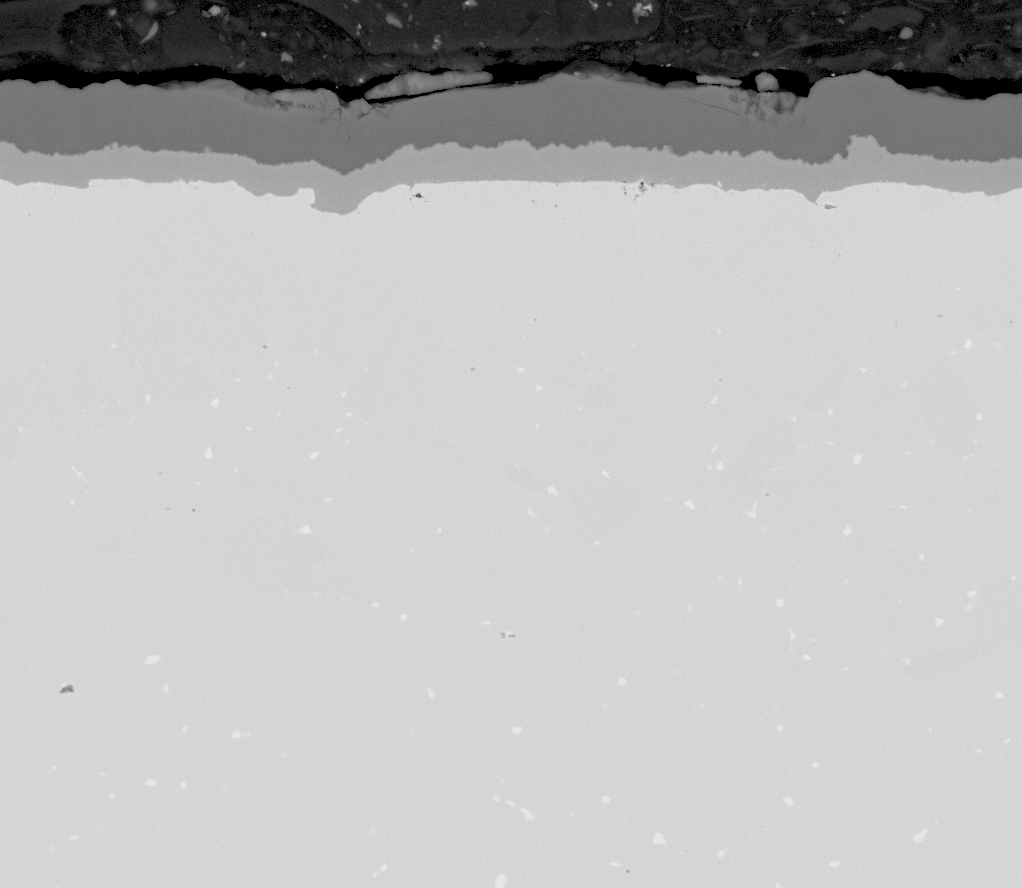
\includegraphics[width=\linewidth]{PICTURES/intro/115.png}
        \caption{Material sample with coating.}
        \label{fig:coating}
    \end{subfigure}
    \hfill
    \begin{subfigure}{0.40\textwidth}
        \centering
        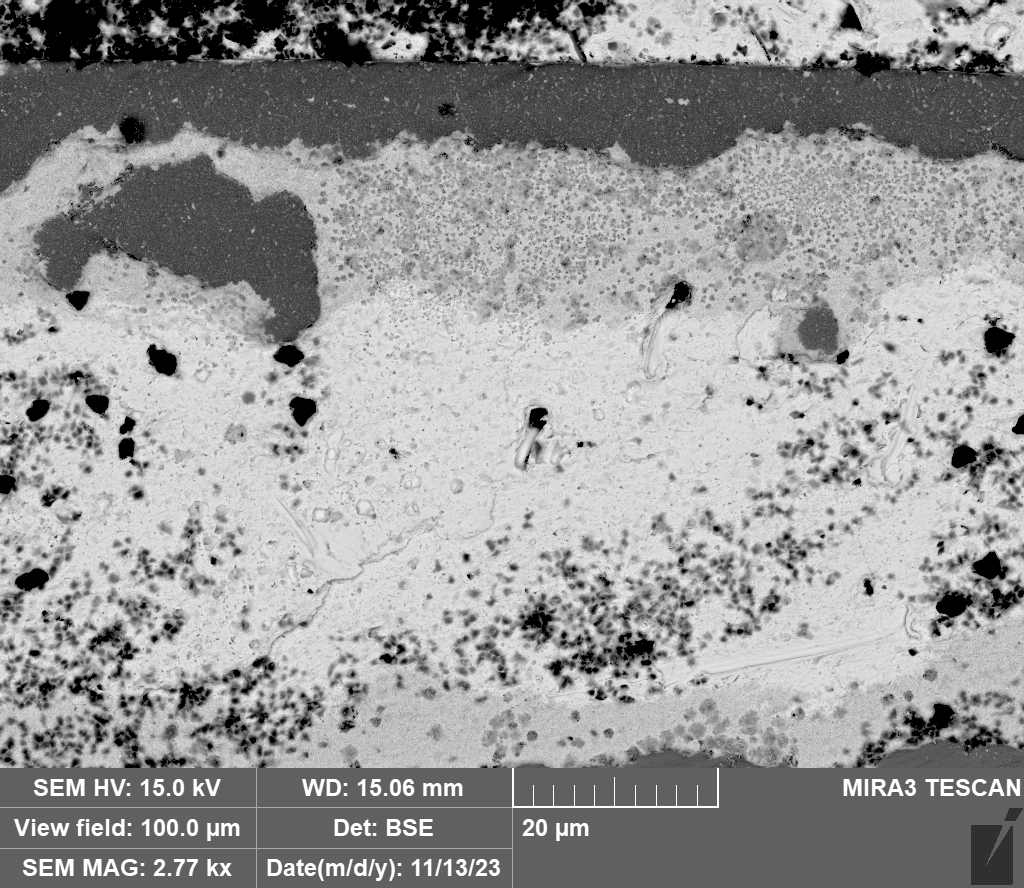
\includegraphics[width=\linewidth]{PICTURES/intro/625_3500h_low_cross_strana1_13.png}
        \caption{Material sample with oxidation.}
        \label{fig:oxidation}
    \end{subfigure}
    \caption{Coating and oxidation layers in the material sample.}
    \label{fig:coating-oxidation}
\end{figure}


